\chapter{Lower bounds for multilinear models}\label{chap:multilinear}

Most of the polynomials that are studied usually, like those described in \autoref{chap:notation}, are multilinear. 
A natural question is whether or not multilinear polynomials can be computed in a ``multilinear fashion''. 
This is formalized by what the model of multilinear circuits, in a way analogous to homogeneous circuits. 

\begin{definition}[Multilinear circuits]
A circuit $C$ is said to be \emph{multilinear} if every gate of the circuit computes a multilinear polynomial. 
A circuit is said to be \emph{syntactically multilinear} if for any $g = g_1 \times g_2$, there is no variable that has a path to both $g_1$ and $g_2$. 
\end{definition}

Note that syntactic multilinearity of course implies multilinearity as the definition forces all gates to compute multilinear polynomials. 
However, we could have a setting where there is a gate $g = g_1 \times g_2$ where some variable $x$ has a path to both $g_1$ and $g_2$ but it so turns out that $g_1$ is independent of $x$ due to other cancellations. 
However, for arithmetic formulas, the two notions are equivalent. 

\begin{exercise}
Given any arithmetic formula $\Phi$ that is multilinear, show that it can be converted to a formula $\Phi'$ of size $\poly(\Phi)$ that is syntactically multilinear. 

\noindent
{\bf (Imp.)} Why does the same not work for multilinear circuits? 
\end{exercise}

This section shall deal mainly with multilinear formulas so we may assume without loss of generality that they are syntactically multilinear. 
Raz \cite{raz2004} showed that multilinear formulas computing the $\Det_n$ or $\Perm_n$ must be of size $n^{\Omega(\log n)}$. 
The complexity measure used by Raz also led to exponential lower bounds for constant depth multilinear circuits \cite{raz-yehudayoff} and super-linear lower bounds for syntactic multilinear circuits \cite{RSY08}. 
\Hrubes and Yehudayoff~\cite{HY11a} then showed a super-polynomial lower bound \emph{homogeneous} multilinear formulas computing the elementary symmetric polynomial.

Although the lower bound of \Hrubes and Yehudayoff was subsequent to the results of Raz and Yehudayoff~\cite{raz2004,raz-yehudayoff}, we shall see their lower bound first which uses a suprisingly simple complexity measure. For the non-homogeneous setting, the complexity measure used here would also be the \emph{rank of the partial derivative matrix} from \autoref{chap:evalDim}. We shall start off with a structural result whenever we are dealing with formulas, which builds on the depth reduction for formulas \autoref{lem:formula-depth-reduction}. 

\section{Log-product representations for formulas}

The following structural lemma shows that any multilinear formula can be converted in to a small sum of \emph{log-product} polynomials. 
The techniques of the following lemma can also be used in other settings with minor modifications, and we shall encounter a different version of this lemma later as well.
These normal forms is from the survey of Shpilka and Yehudayoff~\cite{sy}, and also from the result of \Hrubes and Yehudayoff~\cite{HY11a}. 

\begin{definition}\label{defn:mult-logproduct}
  A multilinear polynomial $f\in \F[X]$ is called a \emph{multilinear log-product} polynomial if $f = g_1\dots g_t$ and there exists a partition of variables $X = X_1 \sqcup \dots \sqcup X_t$ such that
  \begin{itemize}
  \item $g_i \in \F[X_i]$ for all $i \in [t]$.
  \item $\pfrac{1}{3}^i |X| \leq |X_i| \leq \pfrac{2}{3}^i |X|$ for all
    $i$, and $|X_t| = 1$.
  \end{itemize}
\end{definition}

\begin{lemma}\label{lem:mult-logproduct}
  Let $\Phi$ be a multilinear formula of size $s$ computing a polynomial $p$. 
Then $p$ can be written as a sum of $(s+1)$ log-product multivariate polynomials.
\end{lemma}
\begin{proof}
  Similar to \autoref{lem:formula-depth-reduction}, let $v$ be a node in $\Phi$ such that set of variables $X_v$ that it depends on satisfies $\frac{|X|}{3} \leq \abs{X_v} \leq \frac{2|X|}{3}$. 
If $\Phi_v$ is the polynomial computed at this node, then $f$ can be written as
  $$
  f \spaced{=} \Phi_v \cdot g_1 + \Phi_{v=0} \quad\text{for some $g_1 \in \F[X\setminus X_v]$}.
  $$
  where $\Phi_{v=0}$ is the formula obtained by replacing the node $v$ by zero. 
Note that the subtree at the node $v$ is completely disjoint from $\Phi_{v=0}$. 
Hence the sum of the sizes of $\Phi_v$ and $\Phi_{v=0}$ is at most $s$. 
Hence, $g_1 \in \F[X\setminus X_v]$ and $\frac{|X|}{3} \leq \abs{X \setminus X_v} \leq \frac{2|X|}{3}$. 
Inducting on the formulas $\Phi_v$ and $\Phi_{v=0}$ gives the lemma.
\end{proof}

There are many variants of this formula depending on how you pick the node $v$ in the proof above.
Here is another variant that find a node $v$ based on \emph{degree} rather than the number of variables that it depends on.
We state it here without proof but it follows exactly as in the lines of \autoref{lem:mult-logproduct}.

\begin{lemma}\label{lem:hom-logproduct}
  Let $\Phi$ be a homogeneous formula of size $s$ computing a polynomial $p$ of degree $d$.
Then $p$ can be written as a sum of $(s+1)$ \emph{log-product} polynomials, that is,
\[
p \spaced{=} f_1 + \cdots + f_{r}\quad\quad \text{with $r \leq s+1$}
\]
where for each $i \in [r]$, we have $f_i = f_{i1} \cdots f_{i\ell}$ satisfying
\begin{itemize}
\item each $f_{ij}$ is homogeneous,
\item $(1 / 3)^j \cdot d \leq \deg(f_{ij}) \leq (2/ 3)^j \cdot d$,
\item $f_{i\ell} = 1$.
\end{itemize}
In particular, each $f_i$ factors into $\Omega(\log d)$ non-trivial factors of geometrically decreasing degrees. 

Furthermore, if $\Phi$ was a multilinear formula to begin with, then so is the expression on the RHS. 
\end{lemma}


We shall see yet another variant of this trick later in this chapter but we have enough for now to prove the lower bound of \Hrubes and Yehudayoff \cite{HY11a}. 

\section{Lower bounds for homogeneous multilinear formulas}

The main theorem of this section would be the following.

\begin{theorem}[\cite{HY11a}]\label{thm:Hrubes-Yehudayoff}
Any homogeneous multilinear formula that computes the polynomial $\ESym_d$, for $d \leq n/2$, must have size $d^{\Omega(\log d)}$. 
\end{theorem}

The complexity measure used here would be ridiculously simple --- just the number of monomials!
Surprisingly, this is enough to prove the lower bound for homogeneous multilinear formulas. Before we get into the proof, we would need the following approximation for the binomial coefficient. This follows from Stirling's approximation of $n!$. 

\begin{lemma}[Stirling's approximation of $\binom{n}{k}$]\label{lem:stirling-binom} For $n \geq 3k/2$, the following 
\[
\pfrac{1}{3\sqrt{k}} \cdot \pfrac{n^n}{k^k \cdot (n-k)^{n-k}} \spaced{\leq} \binom{n}{k} \spaced{\leq} \pfrac{1}{\sqrt{k}} \cdot \pfrac{n^n}{k^k \cdot (n-k)^{n-k}}
\]
\end{lemma}

\begin{proofof}{\autoref{thm:Hrubes-Yehudayoff}}
If there is a size $s$ homogeneous multilinear formula computing $\ESym_d$, then by \autoref{lem:hom-logproduct} we have an expression of the form
\[
\ESym_d \spaced{=} \sum_{i=1}^{s+1} f_{i1} \cdots f_{i\ell}
\]
with $\ell = \Omega(\log d)$.
We shall show that each multilinear term of the form $f_{i1} \cdots f_{i\ell}$, with geometrically decreasing degrees, can contribute at most $d^{-\Omega(d)} \cdot \binom{n}{d}$ monomials.
This would immediately imply that $s = d^{\Omega(d)}$. \\


Consider a term of the form $f_1 \cdots f_\ell$. Since the degrees drop geometrically, we may assume without loss of generality that $\ell = \Omega(\log d)$ and $\deg(f_i) \geq \sqrt{d}$ (by just multiplying all polynomials of smaller degree together). This is a homogeneous multilinear expression so let $\deg(f_i) = d_i$ and let $f_i$ depend on the variables $X_i$. If $n_i = \abs{X_i}$, then each $f_i$ has at most $\binom{n_i}{d_i}$ monomials. Hence, the total number of monomials from this term is at most
\[
\binom{n_1}{d_1} \cdots \binom{n_\ell}{d_\ell}.
\]
All that's left to do is show that this is significantly smaller than $\binom{n}{d}$. 

\begin{lemma}[\cite{HY11a}]\label{lem:HY-prod-binom}
Let $n\geq 2d$. For any set of non-negative integers satisfying $n_1 + \cdots + n_\ell = n$ and $d_1 + \cdots + d_\ell = d$, we have
\[
\binom{n_1}{d_1} \cdots \binom{n_\ell}{d_\ell} \spaced{\leq} 3 \sqrt{\frac{d}{d_1 \cdots d_\ell}} \cdot \binom{n}{d}
\]
\end{lemma}
The theorem immediately follows from this lemma as each $d_i \geq \sqrt{d}$ and there are $\Omega(\log d)$ of them. 

Before we prove this theorem, let us quickly look at the simpler case when $d = n/2$. In that case, $\binom{n}{d} \approx 2^n / \sqrt{n}$ and the LHS is clearly upper bounded as
\[
\binom{n_1}{d_1} \cdots \binom{n_\ell}{d_\ell} \spaced{\leq} \frac{2^{n_1+ \cdots + n_\ell}}{\sqrt{n_1 \cdots n_\ell}}
\]
giving us a similar bound. The case of general $d$ requires a bit more work but is quite natural (once you know it is true). 

\begin{myproof}{\autoref{lem:HY-prod-binom}}[of \autoref{lem:HY-prod-binom}]
Without loss of generality, we may assume that $n_i \geq 2d_i$ for all $i$. We are trying to understand the following distribution:
\begin{quote}
  If we pick $d$ elements out of $n$ elements, what's the probability that we pick $d_1$ elements from the first $n_1$, and $d_2$ from the next $n_2$ ... etc. 
\end{quote}
The first step is to ask, for fixed values of $n_1, \cdots, n_\ell$, what values of $d_1, \cdots, d_\ell$ maximize this probability. Intuitively, each $d_i$ ought to be proportional to $n_i$ as that is what we would get in expectation. In the perfect regime where $n = \alpha \cdot  d$ and  $n_i = \alpha \cdot d_i$ for each $i \in [\ell]$, we can now use the approximation from \autoref{lem:stirling-binom} to get
\begin{eqnarray*}
\binom{n}{d} & \geq  &  \pfrac{1}{3\sqrt{d}} \cdot \pfrac{n^n}{d^d \cdot (n-d)^{n-d}}\\
 & = & \pfrac{1}{3\sqrt{d}} \cdot \pfrac{d^n \cdot \alpha^n}{d^d \cdot d^{n-d} \cdot (\alpha - 1)^{n-d}}\\
 & = & \pfrac{1}{3\sqrt{d}} \cdot \pfrac{\alpha^n}{(\alpha - 1)^{n-d}}\\
\text{and} \quad\binom{n_i}{d_i} & \leq  &  \pfrac{1}{\sqrt{d_i}} \pfrac{\alpha^{n_i}}{(\alpha - 1)^{n_i-d_i}}\\
\implies \binom{n_1}{d_1} \cdots \binom{n_\ell}{d_\ell}  & \leq & 3 \sqrt{\frac{d}{d_1 \cdots d_\ell}} \cdot \binom{n}{d}
\end{eqnarray*}

To complete the proof, we just have to show that $\binom{n_1}{d_1} \cdots \binom{n_\ell}{d_\ell}$ is maximized when $n_i/d_i \approx n/d$.
To do this, let us consider a term $\binom{n_1}{d_1} \cdot \binom{n_2}{d_2}$ with $d_1/n_1 \gg d_2/n_2$ and show that $\binom{n_1}{d_1 - 1} \cdot \binom{n_2}{d_2 + 1}$ is larger.
This is easy to see because
\begin{eqnarray*}
\frac{\binom{n_1}{d_1 - 1} \cdot \binom{n_2}{d_2 + 1}}{\binom{n_1}{d_1} \cdot \binom{n_2}{d_2}} & = & \frac{d_1 \cdot (n_2 - d_2)}{(n_1 - d_1 + 1) \cdot (d_2 + 1)}\\
 & = & \frac{\pfrac{n_2 + 1}{d_2 + 1} - 1 }{\pfrac{n_1 + 1}{d_1} - 1}\\
 & > & 1.
\end{eqnarray*}
This is still a little incomplete as this ensures that the product is maximized when $d_i$ is as close as possible to $d \cdot (n_i/n)$ but perhaps not quite exactly equal. This can be handled with some minor\footnote{`minor' if one is willing to afford some loss in parameters. But it is also possible to prove the statement claimed with some more work.} changes in the calculation above.  
\end{myproof}

\noindent
The theorem follows immediately from this lemma. 
\end{proofof}

\section{Lower bounds for (non-homogeneous)  multilinear formulas}

Homogeneity is crucially used in the proof of \autoref{thm:Hrubes-Yehudayoff}.
A simple example is just the term $(x_1 + 1) \cdots (x_n + 1)$ which generates every possible multilinear monomial rendering a sparsity based complexity measure completely useless.

However, once again, we can use the \emph{partial derivative matrix} that we studied in \autoref{chap:evalDim} here. In this section, we shall see the lower bounds of Raz \cite{raz2004}, and the lower bound of Raz and Yehudayoff \cite{raz-yehudayoff}. 

\subsection*{Intuition}

A natural first step is to try the simpler task of proving lower bounds for depth-$3$ multilinear circuits. 
$$
f \quad = \ell_{11} \dots \ell_{1d} + \dots + \ell_{s1}\dots \ell_{sd}
$$
The task is now to construct a measure $\Gamma$ such that $\Gamma(\ell_1\dots \ell_d)$ is small whenever each $\ell_i$ is a linear polynomial and different $\ell_i$'s are over disjoint sets of variables. 
Consider the simplest case of $f = (a_1  + b_1x)(a_2  + b_2y)$. 
An observation is that the coefficients of $f$ are given by the $2\times 2$ matrix obtained as $[a_1\ b_1]^T [a_2\ b_2] = \insquare{\begin{array}{cc} a_1a_2 & a_1b_2\\ a_2 b_1 & b_1 b_2\end{array}}$. 
In other words, a polynomial $f = a_0 + a_1x + a_2y + a_3xy$ factorizes into two variable disjoint factors if and only if the matrix $\insquare{\begin{array}{cc} a_0 & a_1\\ a_2 & a_3\end{array}}$ has rank $1$. 
This is another way of reading $f$ as a \emph{non-commutative polynomial}, and this is precisely the partial derivative matrix of $f$ with respect to $\set{x,y} = \set{x} \sqcup \set{y}$ as seen in \autoref{chap:evalDim}. 
\\

\noindent
We recall the definition of the partial derivative matrix with respect to $X = Y \sqcup Z$ from the picture:

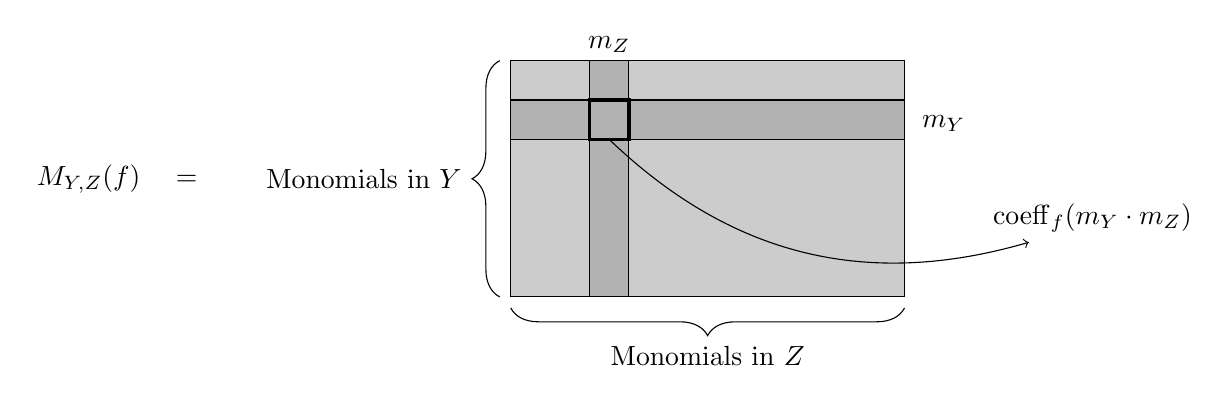
\begin{tikzpicture}
\node at (-5,1.5) {$M_{Y,Z}(f) \quad= $};
\draw[fill=black!20] (0,0) rectangle (5,3);

\draw[decorate,decoration={brace,amplitude=10pt,raise=4pt},yshift=0pt]
(0,0) -- (0,3);
\node[anchor=east] at (-0.5,1.5) {Monomials in $Y$};
\draw[decorate,decoration={brace,amplitude=10pt,mirror, raise=4pt},yshift=0pt] 
(0,0) -- (5,0);
\node[anchor=north] at (2.5,-0.5) {Monomials in $Z$};

\draw[fill=black!30] (1,0) rectangle (1.5,3);
\node at (1.25,3.2) {$m_Z$};

\draw[fill=black!30] (0,2) rectangle (5,2.5);
\node at (5.5,2.2) {$m_Y$};

\draw[very thick] (1,2) rectangle (1.5,2.5);

\node[anchor=west] at (6,1) {$\mathrm{coeff}_f(m_Y \cdot m_Z)$}
edge[<-,bend left] (1.25,2);
\end{tikzpicture}

\noindent
We shall use $\CM{Raz}_{Y,Z}(f)$ to denote the rank of $M_{Y,Z}(f)$. \\


Here are some basic properties of the partial derivative matrix which would be extremely useful in later calculations.

\begin{observation}[Sub-additivity]\label{obs:pdm-subadditivity}
	For any partition $X = Y \sqcup Z$ and any pair of multilinear 
	polynomials $f$ and $g$ in $\FF[X]$ we have 
$\CM{Raz}_{Y,Z}(f+g) \spaced{\leq} \CM{Raz}_{Y,Z}(f) \spaced{+} \CM{Raz}_{Y,Z}(g)$.
\end{observation}
\begin{proof}
Follows from the linearity of the matrix. 
\end{proof}

\begin{observation}[Multiplicativity]\label{obs:pdm-multiplicativity}
If $f_1 \in \F[Y_1,Z_1]$ and $f_2 \in \F[Y_2, Z_2]$ with $Y = Y_1 \sqcup Y_2$ and $Z = Z_1 \sqcup Z_2$, then
$$
\CM{Raz}_{Y,Z}(f_1\cdot f_2) \spaced{=} \CM{Raz}_{Y_1, Z_1}(f_1) \spaced{\cdot} \CM{Raz}_{Y_2, Z_2}(f_2).
$$
\end{observation}
\begin{proof}
  It is not hard to see that $M_{Y,Z}(f_1\cdot f_2)$ is the tensor product $M_{Y_1, Z_1}(f_1) \otimes M_{Y_2, Z_2}(f_2)$, and the rank of a tensor product of two matrices is the product of the ranks.
\end{proof}

\begin{observation}[Multiplication by univariates]\label{obs:pdm-mult-by-univariate}
For any $f \in \F[Y,Z]$ and any $g \in \F[Y]$, if $\F$ is large enough then we have that $\CM{Raz}_{Y,Z}(g \cdot f) \leq \CM{Raz}_{Y,Z}(f)$. 

By symmetry, the same is true when $g \in \F[Z]$. 
\end{observation}
\begin{proof}
  The evaluation dimension of $g \cdot f$ is at most the evaluation dimension of $g$ as any partial evaluation (by evaluating $Y$) of $g \cdot f$ is a scalar times a partial evaluation of $g$.
The observation follows from \autoref{lem:evalDim-to-coeffDim}.
\end{proof}


\begin{observation}[A trivial bound]\label{obs:pdm-upperbound}
For any multilinear polynomial $f$, we have  $\CM{Raz}_{Y,Z}(f) \spaced{\leq} 2^{\min(\abs{Y}, \abs{Z})}$.
\end{observation}
\begin{proof}
  The number of rows is $2^{\abs{Y}}$ and number of columns is $2^{\abs{Z}}$, and hence the rank is upper-bounded by the minimum.
\end{proof}

Let us get back to lower bounds for multilinear models, and attempt to use $\CM{Raz}_{Y,Z}(f)$ defined above. 
Unfortunately, there are examples of simple polynomials like $f = (y_1 + z_1)\dots (y_n + z_n)$ with $\CM{Raz}_{Y,Z}(f) = 2^n$. 
Raz's idea here was to look at $\CM{Raz}_{Y,Z}(f)$ for a \emph{random partition}, and show that with high probability the rank of the partial derivative matrix is far from full. 
As a toy example, we shall see why this has the potential to give lower bounds for depth-$3$ multilinear circuits. 

\begin{lemma}\label{lem:raz-depth-three}
Let $f(X) = \ell_1 \dots \ell_d$ be an $n$-variate multilinear polynomial. 
If $X = Y\sqcup Z$ is a random partition with $|Y| = |Z| = |X|/2$, then with high probability we have
$$
\CM{Raz}_{Y,Z}(f) \quad \leq \quad 2^{|X|/2} \cdot 2^{-|X|/16}.
$$
\end{lemma}

It is to be noted that we should expect a random polynomial to be full-rank with respect to any partition, so the measure $\CM{Raz}_{Y,Z}(f)$ is expected to be $2^{|X|/2}$ which should yield a lower bound of $2^{\Omega(|X|)}$. 

\begin{proof-sketch}
Without loss of generality we can assume that each $\ell_i$ depends on at least two variables as removing the $\ell_i$'s that depend on just one variable does not alter $\CM{Raz}_{Y,Z}(f)$ with respect to any partition. 
Let $|X| = n$. 

Using \autoref{obs:pdm-multiplicativity}, $\CM{Raz}_{Y,Z}(f) \leq 2^d$ and hence if $d < n/3$ then we are done. 
Hence assume that $d \geq n/3$. 
By a simple averaging argument, there must hence be at least $d/4$ of the $\ell_i$'s that depend on at most $3$ variables; we shall refer to these as the \emph{small} $\ell_i$'s. 

Since the partition is chosen at random, on expectation a quarter of the small $\ell_i$'s would have all its variables mapped to either $Y$ or $Z$, hence not contributing to $\CM{Raz}_{Y,Z}(f)$. 
Therefore, with high probability,
$$
\CM{Raz}_{Y,Z}(f) \quad \leq \quad 2^{d} \cdot 2^{-d/16} \spaced{\leq} 2^{n/2} \cdot 2^{-n/16}.
$$
\end{proof-sketch}

More generally, if $f = g_1(X_1)\dots g_t(X_t)$ where the $X_i$'s are mutually disjoint, then a random partition is very unlikely to partition all the $X_i$'s into almost equal parts. 
This naturally calls for using the multilinear log-product representation from \autoref{lem:mult-logproduct} for the case of multilinear formulas. The rest of this section would be proof of Raz's wonderful result \cite{raz2004}. 

\begin{theorem}[\cite{raz2004}] \label{thm:raz-ml-det}
Any multilinear formula computing $\Det_n$ or $\Perm_n$ must be of size $n^{\Omega(\log n)}$. 
\end{theorem}

The proof would be as outlined. If $f$ is computable by a size $s$ multilinear formula, then by \autoref{lem:mult-logproduct} we know that $f$ admits a log-product representation:
\[
f \spaced{=} \sum_{i=1}^{s+1} f_{i1} \cdots f_{i\ell}
\]
Using this, we shall first obtain an upper-bound on $\CM{Raz}_{Y,Z}(f)$ for a random partition $X = Y \sqcup Z$ by showing that any single log-product is far from full-rank. Finally, for $\Det_n$ or $\Perm_n$, we shall prove a lower bound on $\CM{Raz}_{Y,Z}$ for most partitions and that would complete the proof. 

\subsection{Log-products are far from full-rank on a random
  partition}

The main technical part of the proof is to show that log-product multivariate polynomials are far from full-rank under a random partition of variables. 
This would let us show that a sum of log-product multivariate polynomials cannot be full rank unless it is a very large sum.\\

{\bf Main idea: } Suppose $f = g_1 \dots g_t$ where each $g_i \in \F[X_i]$. 
Let $X = Y \sqcup Z$ be a random partition with $|Y| = |Z| = |X|/2$, and $Y_i = Y \intersection X_i$ and $Z_i = Z \intersection X_i$. 
Let $d_i = \abs{\frac{|Y_i| - |Z_i|}{2}}$ measure the imbalance between the sizes of $Y_i$ and $Z_i$, and we shall say $X_i$ is $k$-imbalanced if $d_i \geq k$. 
Let $b_i = \frac{|Y_i| + |Z_i|}{2} = \frac{|X_i|}{2}$.

By \autoref{obs:pdm-multiplicativity}, we know that 
\begin{eqnarray*}
\CM{Raz}_{Y,Z}(f) & = & \CM{Raz}_{Y_i,Z_i}(g_1) \dots \CM{Raz}_{Y_i,Z_i}(g_t)\\
 & \leq & 2^{\min(|Y_1|,|Z_1|)} \cdots  \cdot 2^{\min(|Y_t|,|Z_t|)}\\ 
 & = & 2^{b_1  - d_1} \cdots 2^{b_t - d_t} = \frac{2^{|X|/2}}{2^{d_1 + \dots + d_t}}.
\end{eqnarray*}

Hence, even if one of the $X_i$'s is a little imbalanced, then the product is far from full-rank. \\

\autoref{lem:mult-logproduct} shows that the size of $X_i$ decreases slowly with $i$, and it is not hard to show that $\abs{X_i} \geq \sqrt{\abs{X}}$ for $i \leq t'\eqdef\frac{\log{\abs{X}}}{100}$. 
We wish to show that the probability that none of $g_i$ (for $i\leq t'$) is $k$-unbalanced for $k = \abs{X}^{1/20}$ is very small. 
Let $\mathcal{E}_i$ be the event that $X_i$ is not $k$-unbalanced. 
The goal is to upper bound the probability that all the events $\mathcal{E}_i$ hold. 
These probability calculations would follow from this lemma about the \emph{hypergeometric distribution}.\\

{\bf Hypergeometric Distribution: } Fix parameters $n, g, r \geq 0$, and let $G \subseteq [n]$ with $|G| = g$. 
Informally, the hypergeometric distribution is the distribution obtained on the intersection sizes of a random set of size $r$ with a fixed set of size $g$ from a universe of size $n$. 
Formally, the random variable $\mathcal{H}(n,g,r)$ is defined as:
$$
\Pr\insquare{\mathcal{H}(n,g,r) = k} \spaced{=} \Pr_{R\subseteq [n],|R| = r}\insquare{\abs{R \intersection G} = k} = \frac{\binom{g}{k}\binom{n-g}{r-k}}{\binom{n}{r}}.
$$


The following lemma shows that for a fairly large range of parameters, the hypergeometric distribution does not put too much mass on any value.

\begin{lemma}\label{lem:hypergeom_low-weight}
  Let $n,g,r$ be parameters such that $\frac{n}{4} \leq r \leq \frac{3n}{4}$ and $0\leq g\leq \frac{2n}{3}$. 
Then for any $t\leq g$,
  $$
  \Pr\insquare{\mathcal{H}(n,g,r) = t} \spaced{\leq} O\inparen{\frac{1}{\sqrt{g}}}.
  $$
\end{lemma}
The proof of this lemma follows from standard binomial coefficient estimates on the probability.\\

Let us go back to estimating the probability that all the events $\mathcal{E}_i$ hold.
\begin{eqnarray*}
  \Pr\insquare{\mathcal{E}_1 \wedge \dots \wedge \mathcal{E}_{t'}} & = & \Pr[\mathcal{E}_1] \cdot \Pr[\mathcal{E}_2 \mid \mathcal{E}_1] \cdots \Pr[\mathcal{E}_{t'}\mid \mathcal{E}_1 \wedge \dots \wedge \mathcal{E}_{t'-1}].
\end{eqnarray*}
The event $\mathcal{E}_1$ is just the probability that a random set $Y$ of size $|X|/2$ intersects $X_1$ in $t$ places where $t \in \insquare{\frac{|X_i|}{2} -k , \frac{|X_i|}{2} +k}$. 
This is just a particular setting of the hypergeometric distribution and \autoref{lem:hypergeom_low-weight} asserts that
$$
\Pr[\mathcal{E}_1] \spaced{\leq} O\inparen{\frac{2k}{\sqrt{|X_1|}}} \spaced{\leq} O\inparen{\frac{2k}{\sqrt[4]{|X|}}}.
$$
To apply a similar bound for the other terms, consider the event $\mathcal{E}_i$ given that $\mathcal{E}_1, \dots, \mathcal{E}_{i-1}$ hold. 
Let $X' = X \setminus (X_1 \union \dots \union X_{i-1})$ and $Y' = Y\intersection X'$. 
The fact that $\mathcal{E}_1,\dots, \mathcal{E}_{i-1}$ hold means that the partition has been fairly balanced in the first $(i-1)$ parts and hence $|Y'| \leq \frac{|X'|}{2} + ik$. 
Hence, we would still be in the range of parameters in \autoref{lem:hypergeom_low-weight} to also get that
\begin{eqnarray*}
  \forall i\leq t'\quad \Pr[\mathcal{E}_i\mid \mathcal{E}_1 \wedge \cdots \wedge \mathcal{E}_{i-1}] &\leq& O\inparen{\frac{2k}{\sqrt[4]{|X|}}}\\
  \implies \Pr\insquare{\mathcal{E}_1\wedge \dots \wedge \mathcal{E}_{t'}} & \leq & \abs{X}^{-\epsilon \log \abs{X}} \quad\text{for some $\epsilon > 0$}  \\
  \implies \Pr\insquare{\CM{Raz}_{Y,Z}(g_1\dots g_t) > 2^{(|X|/2) - |X|^{1/20}}} & \leq & \abs{X}^{-\epsilon \log \abs{X}}.
\end{eqnarray*}

\begin{sloppy}
	Hence, if $g_1\dots g_t$ is a log-product multilinear polynomial, 
	then with probability at least $\inparen{1 - |X|^{-\epsilon \log |X|}}$ 
	we have that $\CM{Raz}_{Y,Z}(g_1\dots g_t) \leq 2^{(|X|/2) - |X|^{1/20}}$. 
	Further, if $f$ is computable by a multilinear formula of size $s$ then, 
	by \autoref{lem:mult-logproduct}, $f$ can be written as a sum of 
	$(s+1)$ log-product multilinear polynomials. 
Hence, with probability 
	at least $\inparen{1 - (s+1)|X|^{-\epsilon \log |X|}}$ we have that
		$$\CM{Raz}_{Y,Z}(f) \spaced{\leq} (s+1) \cdot 2^{(|X|/2) - |X|^{1/20}}. $$
	Hence, if $(s+1) < |X|^{(\epsilon/2) \log |X|}$, then with high 
	probability a random partition would ensure 
	$\CM{Raz}_{Y,Z}(f) \ll 2^{|X|/2}$. 
Let us record this as a lemma.
\end{sloppy}

\begin{lemma}\label{lem:multformula-lowrank}
  Let $f \in \F[X]$ be computed by a multilinear formula of size $s < |X|^{(\epsilon/2) \log |X|}$ for a small enough constant $\epsilon > 0$. 
Then with probability at least $(1 - |X|^{-(\epsilon/2)\log |X|})$ we have $$\CM{Raz}_{Y,Z}(f) \spaced{\leq} (s+1)\cdot 2^{|X|/2} \cdot 2^{-|X|^{1/20}}$$ for a random partition $X = Y \sqcup Z$ with $|Y| = |Z| = |X|/2$.
\end{lemma}

\subsection{$\Det_n$ and $\Perm_n$ have large rank}

The last step of the proof would be to find an explicit polynomial whose partial derivative matrix under a random partition has large rank. 
As earlier, our candidate polynomial would be $\Det_n$ or $\Perm_n$. 
Unfortunately, both these polynomials are over $n^2$ variables and degree $n$. 
It is not hard to verify that the rank of the partial derivative matrix of $\Det_n$ or $\Perm_n$ can never be greater than $2^{2n}$. 
Hence directly using \autoref{lem:multformula-lowrank}, we would have $2^{O(n)}$ competing with $2^{n^2/2 - n^{O(1)}}$ which is simply futile. 
A simple fix is to first randomly restrict ourselves to fewer variables and then apply \autoref{lem:multformula-lowrank}. 

Let $m = n^{1/3}$. 
Let $\sigma$ be a random restriction that assigns random values to all but $2m$ randomly chosen variables. 
We shall call this set of $2m$ variables as $X$, and randomly partition this into two sets $Y$ and $Z$ of size $m$ each. 
Hence, $\sigma(\Det_n)$ reduces to a multilinear polynomial over $2m$ variables. 
It is also worth noting that a multilinear formula remains a multilinear formula under this restriction. 
The following claim is easy to verify. 

\begin{claim}
With probability at least $1/2$, the variables in $X$ belong to distinct rows and columns. 
\end{claim}

We shall restrict ourselves to only these random restrictions, and without loss of generality let the sets be $Y = \inbrace{x_{1,1},x_{3,3},\dots,x_{2m-1,2m-1}}$ and $Z = \inbrace{x_{2,2},x_{4,4},\dots, x_{2m,2m}}$. 
For ease of notation, we shall refer to $x_{2i-1,2i-1}$ as $y_i$ and $x_{2i,2i}$ as $z_i$ for $i = 1,\dots, m$. 

Consider the following restriction:
\begin{eqnarray*}
f & = & \Det \insquare{ \begin{array}{cccccccc}
y_1 & 1   &        &     &     &  &        &   \\
1   & z_1 &        &     &     &  &        &   \\
    &     & \ddots &     &     &  &        &   \\
    &     &        & y_m &1    &  &        &   \\
    &     &        & 1   &z_m  &  &        &   \\
    &     &        &     &     & 1&        &   \\
    &     &        &     &     &  & \ddots &   \\
    &     &        &     &     &  &        & 1
  \end{array}}\\
 &= & (y_1z_1 - 1)\dots (y_mz_m - 1).
\end{eqnarray*}
It is easy to check that $\CM{Raz}_{Y,Z}(f) = 2^m$. 
Although this is a single restriction with large rank, the Schwartz-Zippel-DeMillo-Lipton lemma immediately gives that random restriction would also have rank $2^m$ with high probability\footnote{provided the underlying field is large, but this isn't really a concern as we can work with a large enough extension if necessary}. 
We shall record this as a lemma. 

\begin{lemma}\label{lem:det-raz-lowerbound}
With probability at least $1/100$, we have that $\CM{Raz}_{Y,Z}(\sigma(\Det_n)) = 2^m$ where $\sigma$ is a random restriction to $2m$ variables for $m = n^{1/3}$. 
\end{lemma}


Combining \autoref{lem:det-raz-lowerbound} with \autoref{lem:multformula-lowrank}, we have the following theorem. 

\begin{theorem}[\cite{raz2004}] Any multilinear formula computing $\Det_n$ or $\Perm_n$ must be of size $n^{\Omega(\log n)}$. \qed
\end{theorem}

\subsection{Constructing a full-rank polynomial}\label{sec:fullrankpoly}

As alluded to earlier,  if $f$ is a random polynomial, then for any partition $X = Y \sqcup Z$ with $|Y| = |Z| = |X|/2$ we expect $\CM{Raz}_{Y,Z}(f) = 2^{|X|/2}$. 
Can we construct such a polynomial explicitly? 
This was first answered by Raz~\cite{Raz06}, and the construction was later simplified by Raz and Yehudayoff~\cite{ry08} and we shall describe the latter here. \\

{\bf Main idea:} Suppose you know the partition as $Y = \inbrace{y_1,\dots, y_n}$ and $Z = \inbrace{z_1,\dots, z_n}$, then building a polynomial such that $M_{Y,Z}(f)$ is full-rank is easy --- just take $f = (y_1z_1 + 1)\dots (y_n z_n + 1)$ which makes $M_{Y,Z}(f)$ the identity matrix. 
What we would like is to have one such copy for every partition, and we would also like to build it in a way so that $f$ can be computed in $\VP$. \\

The first attempt is to build the polynomial inductively for every partition into two equal parts, but ``remembering'' partial partitions take too much memory (similar to the situation we had in \autoref{thm:det-abp}). 
Raz and Yehudayoff instead use a different construct that, rather than being based on partitions, is instead based on Dyck-strings or well-matched parentheses. 

The language $\mathrm{Dyck}(n)$ refers to strings of length $2n$ over symbols `$($' and `$)$' that is well-matched in the natural way. 
That is ``()()'' and ``(())'' belong to $\mathrm{Dyck}(2)$ but not ``())(''. 
Raz and Yehudayoff come up with a natural map to convert every such string to a full-rank polynomial, and we shall just state this by example. 
\begin{eqnarray*}
\Omega(\text{``(())''}) & = & (x_1x_4 + 1)\cdot (x_2x_3 + 1)\\
\Omega(\text{``()()''}) & = & (x_1x_2 + 1)\cdot (x_3x_4 + 1)
\end{eqnarray*}
That is, if the opening bracket at position $i$ is closed at position $j$, then there is a factor $(x_ix_j + 1)$. 
Let us define the polynomial as follows:
\[
f(x_1,\dots, x_{2n}) \spaced{=} \sum_{s\in \mathrm{Dyck}(n)} \Omega(s) 
\]
Let us attempt to compute the polynomial using a small circuit in the following natural inductive manner. 
\[
f_{i,j}(\vecx) \spaced{=} \begin{cases}
(x_ix_j+1) & \text{if $j = i+1$}\\
0 & \text{if $j-i$ is even}\\
(x_ix_j+1) \cdot f_{i+1,j-1} &\\
 \spaced{+} \sum\limits_{r=i+1}^{j-1} f_{i,r}\cdot f_{r+1,j} & \text{otherwise}
\end{cases}
\]
However, $f_{1,2n}$ is \emph{not equal} to the polynomial $f$ as the term corresponding to ``()()()$\dots$()'' has coefficient $1$ in $f$ but is $C_n$, the $(n-1)$-th Catalan number. 
Nevertheless, this inductively defined polynomial $f_{1,2n}$ has most of the properties we need. 
Raz and Yehudayoff take a slight variant of it by adding a few auxiliary variables $\inbrace{\omega_{i,j,k}}$ to build the following polynomial over the field $\F(\inbrace{\omega_{i,j,k}})$. 
\[
\tilde{f}_{i,j}(\vecx) \spaced{=} \begin{cases}
(x_ix_j+1) & \text{if $j = i+1$}\\
0 & \text{if $j-i$ is even}\\
(x_ix_j+1) \cdot \tilde{f}_{i+1,j-1} &\\
 \spaced{+} \sum\limits_{r=i+1}^{j-1} \tilde{f}_{i,r}\cdot \tilde{f}_{r+1,j} \cdot \omega_{i,r,j} & \text{otherwise}
\end{cases}
\]

\begin{lemma}[\cite{ry08}]\label{lem:fullrankpoly}
The polynomial $\tilde{f} = \tilde{f}_{1,2n}$ has the property that for every $X = Y \sqcup Z$ with $|Y| = |Z| = |X|/2$ we have $\CM{Raz}_{Y,Z}(\tilde{f}) = 2^{|X|/2}$. 
\end{lemma}
\begin{proof}
The proof shall be over induction on $n$. 
For the base case, statement is obviously true for $n = 1$ as $\tilde{f} = (x_1x_2 + 1)$ in this case. 

Suppose $n > 1$, and let $X = Y \sqcup Z$ be any partition with $|Y| = |Z| = |X|/2$. 
Then, either both $x_1$ and $x_{2n}$ belong to the same side of the partition, or they belong to different sides. 
Let us handle each case separately. 

\begin{description}
\item{Case 1:  $x_1$ and $x_{2n}$ are in different parts}. 

Then, polynomial $\tilde{f}$ where we set $\omega_{1,i,2n} = 0$ for all $i$. 
Under this substitution, $\tilde{f}$ is equal to $(x_1x_{2n}+ 1)\cdot \tilde{f}_{2,2n-1}$. 
By induction, we know that $\tilde{f}_{2,2n-1}$ is full-rank under equal sized partition and hence so is $(x_1 x_{2n} + 1) \cdot \tilde{f}_{2,2n-1}$. 
As setting variables to zero can only reduce the rank, it follows that $M_{Y,Z}(\tilde{f})$ must be full-rank as well. 

\item{Case 2:  $x_1$ and $x_{2n}$ are in the same part}. 

Since $|Y| = |Z| = |X|/2$, there must be some intermediate point $r$ such that the two intervals $[1,r]$ and $[r+1,2n]$ are both split evenly by $Y$ and $Z$. 
Using induction on each of these smaller intervals again, we get that $M_{Y,Z}(\tilde{f})$ is full-rank again. 
\end{description}
\end{proof}

This is one of the very few polynomials that we are aware of that can be computed by polynomial sized arithmetic circuits, but is not known to be computable by polynomial size ABPs. 

\section{Stronger lower bounds for constant depth multilinear formulas}

Looking back at \autoref{lem:multformula-lowrank}, we see that whenever $f(X)$ is computable by a size $s$ multilinear formula $\CM{Raz}_{Y,Z}(f)$ is exponentially smaller than $2^{|X|/2}$ with probability $\inparen{1 - s\cdot |X|^{-\epsilon \log |X|}}$. 
Hence we had to settle for a $n^{\Omega(\log n)}$ lower bound not because of the rank deficit but rather because of the bounds in the probability estimate. 
Unfortunately, this lower bound technique cannot yield a better lower bound for multilinear formulas as we have already seen (in \autoref{sec:fullrankpoly}) that there are explicit examples of polynomials computable by poly-sized multilinear circuits with $\CM{Raz}_{Y,Z}(f) = 2^{|X|/2}$ under \emph{every} partition. 
However, the probability bound can be improved in the case of constant depth multilinear circuits to give stronger lower bounds. 


Note that \autoref{lem:multformula-lowrank} was proved by considering \emph{multilinear log-products} (\autoref{defn:mult-logproduct}) as the building blocks. 
To show that a multilinear log product $g_1(X_1)\dots g_{\ell}(X_\ell)$ has small rank under a random partition, we argued that the probability that all the $X_i$'s are partitioned in a roughly balanced fashion is quite small. 
This was essentially done by thinking of this as $\ell = O(\log n)$ close-to-independent events, each with probability $1/\mathrm{poly}(n)$. 

If $\ell$ was much larger than $\log n$ (with other parameters being roughly the same), it should be intuitively natural to expect a much lower probability of all the $X_i$'s being partitioned in a roughly balanced manner. 
This indeed is the case for constant depth multilinear circuits, and we briefly sketch the key points where they differ from the earlier proof. 
The first is an analogue of \autoref{defn:mult-logproduct} in this setting. 

\begin{definition}\label{defn:mult-t-prod}
A multilinear polynomial $f$ is said to be a \emph{multilinear $t$-product} if $f$ can be written as $f = g_1\dots g_t$ with the following properties:
\begin{itemize}
\item The variable sets of the $g_i$ are mutually disjoint
\item Each $g_i$ non-trivially depends on at least $t$ variables
\end{itemize}
\end{definition}

\begin{lemma}\label{lem:mult-t-prod-rep}
Let $f$ be a multilinear polynomial of degree $d$ over $n$ variables that is computed by a depth-$\Delta$ multilinear formula $\Phi$ of size $s$. 
Then, $f$ can be written as a sum of at most $s$ multilinear $t$-products for $t = \inparen{n/100}^{1/2\Delta}$, and a multilinear polynomial of degree at most $n/100$.  
\end{lemma}
\begin{proof}
If $d < n/100$, then the lemma is vacuously true. 
Since $\Phi$ is a formula of depth $\Delta$ and computes a polynomial of degree $d > n/100$, there must be at least one product gate $v$ of fan-in at least $\inparen{\frac{n}{100}}^{1/\Delta} = t^2$. 
Then similar to \autoref{lem:mult-logproduct}, 
$$
f \quad=\quad \Phi_v \cdot f'  + \Phi_{v=0}
$$
As $\Phi_v$ is a product of $t^2$ polynomials, by grouping the factors together we have that $\Phi_v \cdot f'$ is a multilinear $t$-product. 
Further, $\Phi_{v=0}$ is a multilinear polynomial that is computable by a depth-$\Delta$ formula of smaller size and we can induct on $\Phi_{v=0}$. 
\end{proof}

\begin{lemma}\label{lem:mult-const-depth-upper-bound}
Let $f(X)$ be an $n$-variate polynomial computed by a depth-$\Delta$ multilinear formula of size $s$. 
If $X = Y \sqcup Z$ is a randomly chosen partition with $|Y| = |Z| = n/2$, then with probability at least $(1 - s \cdot \exp({-n^{\Omega(1/\Delta)}}))$ we have
$$
\CM{Raz}_{Y,Z}(f) \quad\leq\quad (s+1) \cdot 2^{n/2} \cdot \exp(-n^{\Omega(1/\Delta)}).
$$
\end{lemma}
\begin{proof-sketch}
By \autoref{lem:mult-t-prod-rep}, we have that $f$ can be written as $g_0 + g_1 + \dots + g_s$ where $\deg(g_0) \leq n/100$ and $g_1,\dots, g_s$ are multilinear $t$-products. 
Note that since $g_0$ is a multilinear polynomial of degree at most $(n/100)$, the number of monomials in $g_0$ is at most $\binom{n}{n/100} \leq 2^{n/10}$. 
Hence, $\CM{Raz}_{Y,Z}(g_0) \leq 2^{n/10}$. 

For the other $g_i$'s, we can bound the probability that $\CM{Raz}_{Y,Z}(g_i)$ is large in a very similar fashion as in \autoref{lem:multformula-lowrank}, as the probability that all the factors of $g_i$ are partitioned in a balanced manner is roughly the intersection of $t$ independent events. 
By very similar estimates, this probability can be bounded by $(1/\mathrm{poly}(n))^t$. 
Hence, with high probability 
$$
\CM{Raz}_{Y,Z}(f) \spaced{\leq} \CM{Raz}_{Y,Z}(g_0) + \dots + \CM{Raz}_{Y,Z}(g_s) \spaced{\leq} (s+1)\cdot 2^{n/2} \cdot \exp(-n^{\Omega(1/\Delta)}).
$$
\end{proof-sketch}

Combining \autoref{lem:mult-const-depth-upper-bound} with \autoref{lem:det-raz-lowerbound}, we have the following theorem of Raz and Yehudayoff. 

\begin{theorem}[\cite{raz-yehudayoff}]
Any multilinear formula of depth $\Delta$ computing $\Det_n$ or $\Perm_n$ must be of size $\exp(n^{\Omega(1/\Delta)})$.  \qed
\end{theorem}

\section{Extending to non-multilinear depth-three circuits}

Recall that a multilinear depth three circuit is a sum of \emph{multilinear terms} that are polynomials of the form $T = \ell_1 \dots \ell_d$ where every variable $x \in X$ is present in at most one $\ell_i$. 
Kayal and Saha \cite{ks15} study more general depth three circuits that are sums of terms where very variable occurs in ``few'' linear factors. 

\begin{definition}[Multi-$k$-ic depth three circuits]
  A product of linear polynomials $T = \ell_1 \dots \ell_d$ is said to be a \emph{multi-$k$-ic term} if every variable $x \in X$ occurs in at most $k$ of the linear polynomials. 
A depth three circuit is said to be a \emph{multi-$k$-ic depth three circuit} if it is a sum of multi-$k$-ic terms. 
\end{definition} 

For example, the circuit computing $(x_1 + x_2)(x_2 + x_3)(x_1 +x_3) + (x_1 + x_3)(x_2 + 3x_3)$ multi-$2$-ic circuit. \\

Kayal and Saha \cite{ks15} studied the question of proving lower bound for such multi-$k$-ic depth-three circuits for small $k$ and they showed that the techniques of \cite{raz2004} can be generalized to give exponential lower bounds for multi-$k$-ic depth-three circuits for small $k$. 

\begin{theorem}[\cite{ks15}]\label{thm:multi-k-ic} There is an explicit $n$-variate polynomial $f \in \VNP$ such that any multi-$k$-ic depth-three circuit computing it must have size $2^{\Omega(n/2^{100k})}$. 
\end{theorem}

\subsubsection*{Revisiting the measure}

In all the multilinear lower bounds we saw, the measure used was the rank of the partial derivative matrix under a random partition. 
We shall use the same measure, but keeping in mind that monomials could be non-multilinear. 
Once again, for a partition $X = Y \sqcup Z$, we shall define the matrix $M_{Y,Z}(f)$ to be the matrix whose rows are indexed by all (possibly non-multilinear) monomials $m_i$ in the $Y$ variables, and columns are indexed by all (possibly non-multilinear) monomials $m_j$ in the $Z$ variables with the entry being the coefficient of $m_i m_j$ in $f$. 
We shall abuse notation and use $\CM{Raz}_{Y,Z}(f)$ to refer to the rank of $M_{Y,Z}(f)$. 

As in the earlier lower bounds, we shall take a random partition $X = Y \sqcup Z$ and study $\CM{Raz}_{Y,Z}(f)$ for a small multi-$k$-ic circuit. 

\begin{remark*}\rm 
We shall take a slight deviation from the way we chose partitions earlier. 
Here, we shall take every variable $x\in X$ and map it to $Y$ or $Z$ with equal probability. 
Thereby, it is possible that $|Y|$ is not exactly $|X|/2$ but it would nevertheless be close to it with high probability. 
This modification gives us the useful feature that the random partition is made of independent events. 
This would turn out to be useful in the following calculations. 
\end{remark*}

\subsection*{Proof of Theorem~\ref{thm:multi-k-ic}}

The proof strategy will be the same as earlier. 
For a random polynomial with degree in every variable bounded by $k$, we expect $\CM{Raz}_{Y,Z}(f)$ to be $\Omega(k^{\min(|Y|,|Z|)})$. 
We shall show that for a multi-$k$-ic term $T = \ell_1\dots \ell_d$, under a random partition $X = Y \sqcup Z$, the measure $\CM{Raz}(T)$ will be far from $k^{n/2}$ with high probability, if $n = |X|$. 

The proof that we shall describe here is a simplification of the original proof of \cite{ks15}. 
This proof would be very similar to the proof of \autoref{lem:raz-depth-three}. 

\begin{lemma}\label{lem:multi-k-ic-ub}
Let $X = Y \sqcup Z$ be a random partition. 
If $T$ is a multi-$k$-ic term, then with probability $\inparen{1 - \exp(-\frac{|X|}{2^{6k+1}})}$
\[
\CM{Raz}_{Y,Z}(f) \spaced{\leq} (1+k)^{\min(|Y|,|Z|)}\cdot \exp\inparen{-\frac{|Y|}{2^{3k+1}}}
\]
\end{lemma}


Let us quickly recall how the proof of \autoref{lem:raz-depth-three} proceeded. 
We essentially showed that for any linear polynomial involving ``few'' variables, with some non-trivial probability the random partition would map all the variables to one side of the partition. 
Thus, if there are many such linear polynomials, the is a large fraction of the linear polynomials that do not contribute to $\CM{Raz}_{Y,Z}(T)$. 
If there are very few such ``small'' linear polynomials, then the degree would have cannot be too large and we can use a trivial bound. 
The proof here shall proceed in a very similar fashion. 


\begin{proofof}{\autoref{lem:multi-k-ic-ub}}
Let $T = \ell_1 \dots \ell_d$. 
We shall call a factor $\ell$ to be ``large'' if the number of variables it depends on is at least $3k$, and let $T_L$ be the product of all $\ell_i$'s that are ``large'', and let $T_S$ be the product of the remaining $\ell_i$'s. 


\autoref{obs:pdm-multiplicativity}, generalized to this setting, gives that $\CM{Raz}_{Y,Z}(T) \leq \CM{Raz}_{Y,Z}(T_L) \cdot \CM{Raz}_{Y,Z}(T_S)$. 
Thus, it suffices to bound each term separately. 
The easy case is, as one would expect, handling $T_L$. 
Suppose $Y$ is the smaller of the sets $Y$ and $Z$. 
Let us list down every variable in $Y$ that occurs in $T_L$ in order as $y_1,\dots, y_{r_L}$ (with repetition). 
Let $r_L = (1-\delta) |Y|k$ for some $0\leq \delta \leq 1$. 
A trivial bound for $\CM{Raz}_{Y,Z}(T_L)$ is 
\begin{equation}\label{eqn:TL-bound}
\CM{Raz}_{Y,Z}(T_L)\spaced{\leq} 2^{\deg(T_L)} \spaced{\leq} 2^{r_L/3k} \spaced{\leq} 2^{(1-\delta)|Y|/3}
\end{equation}
The trickier case is with $T_S$ but intuitively the setting is very similar to what we encountered in the proof of \autoref{lem:raz-depth-three}. 
Since any factor $\ell$ of $T_S$ depends on at most $3k$ variables, with probability at least $\inparen{\frac{1}{2^{3k-1}}}$, all the variables of $\ell$ would be on the same side of the partition. 
Thus, on expectation, there would be at least $\inparen{\frac{\deg(T_S)}{2^{3k-1}}}$ factors that would not contribute to $\CM{Raz}_{Y,Z}(T_S)$ at all. 
In \autoref{lem:raz-depth-three}, we could show that the number of such factors is concentrated around the expectation since the linear polynomials were disjoint and the events were independent. 
However, in this setting a variable can occur in multiple factors. 
Nevertheless, one can still use the fact that every variable occurs in at most $k$ factors to establish a concentration very similar to Chernoff's Bounds. 
The following beautiful theorem of Gavinsky, Lovett, Saks and Srinivasan \cite{GLSS12} is exactly what we need. 

\begin{theorem}[\cite{GLSS12}]
Let $X_1,\dots, X_n$ be independent random variables. 
Let $E_1,\dots, E_r$ be boolean random variables that are functions of $\inbrace{X_i}$ such that each $X_i$ influences at most $k$ of the $E_j$'s. 
If $\Pr[E_i = 1] \geq p$, then for any $\epsilon > 0$, we have
\[
\Pr\insquare{E_1 + \dots + E_r  \spaced{\leq} (p - \epsilon) r } \spaced{\leq} e^{-2\epsilon^2 r/k}
\]
\end{theorem}

Again, let us list down every variable in $Y$ that occurs in $T_S$ in order as $y_1,\dots, y_{r_S}$ (listed with repetition). 
Note that $r_S + r_L \leq |Y|k$, and since $r_L = (1-\delta)k|Y|$,  we have that $r_S \leq \delta |Y|$. 
Let $E_i$ be the indicator random variable that is $1$ if all the variables of the factor  $\ell$ that contains $y_i$ are mapped to the same side of the partition; we shall call such an instance variable $y_i$ as \emph{ineffective}. 
In other words, the set of ineffective instances $y_i$ (with $E_i = 1$) are those that do not contribute to $\CM{Raz}_{Y,Z}(T_S)$. 

Since each $\ell$ depends on at most $3k$ variables, we have that $\Pr[Y_i = 1] \geq  p= \frac{1}{2^{3k-1}}$. 
Let us set $\epsilon = \frac{p}{2}$ and use the above theorem. 
Hence, the probability at least $\inparen{1 - \exp(-\frac{r_S}{k2^{6k}})}$, there are at least $\inparen{\frac{r_S}{2^{3k}}}$ ineffective instances. 

For every variable $x \in Y$, let $d_x$ be the number of occurrences of $x$ that is not ineffective. 
We know that $\sum_{x\in Y} d_x \leq r_S \cdot \inparen{1 - \frac{1}{2^{3k}}}$. 
On the other hand, $\prod_{x\in Y} (1 + d_x)$ is an upper-bound on the number of non-zero rows of $M_{Y,Z}(T_S)$. 
Hence,
\begin{eqnarray*}
\CM{Raz}_{Y,Z}(T_S) \spaced{\leq}\prod_{x\in Y} (1 + d_i) & \leq & \inparen{\frac{\sum_{x\in Y} (1 + d_x)}{|Y|}}^{|Y|}\\
 & \leq & \inparen{\frac{|Y| + r_S \inparen{1 - \frac{1}{2^{3k}}}}{|Y|}}^{|Y|}\\
 & \leq & \inparen{1 + \delta k\inparen{1 - \frac{1}{2^{3k}}}}^{|Y|}\\
 & \leq & \inparen{1+\delta k}^{|Y|} \cdot \inparen{1 - \frac{1}{2^{3k+1}}}^{|Y|}\\
 & \leq & \inparen{1+k}^{\delta |Y|}\exp\inparen{-\frac{|Y|}{2^{3k+1}}}
\end{eqnarray*}
Combining this with \eqref{eqn:TL-bound}, we get with probability at least $\inparen{1 - \exp(-\frac{|X|}{2^{6k+1}})}$
\[
\CM{Raz}_{Y,Z}(T) \spaced{\leq} (1+k)^{\min(|Y|,|Z|)}\cdot \exp\inparen{-\frac{|Y|}{2^{3k+1}}}
\]
\end{proofof}

\noindent
Using an union bound over all multi-$k$-ic terms, we obtain the simple corollary. 

\begin{corollary}\label{cor:multi-k-ic-ub}
Let $C = T_1 + \dots + T_s$ be a multi-$k$-ic circuit over variables $X$. 
Then for a random partition $X = Y \sqcup Z$, with probability at least $\inparen{1 - s  \cdot \exp(-\frac{|X|}{2^{6k+1}})}$, we have
\[
\CM{Raz}_{Y,Z}(C) \spaced{\leq} s \cdot (1+k)^{\min(|Y|,|Z|)}\cdot \exp\inparen{-\frac{|Y|}{2^{3k+1}}}
\]
In particular, if $s < \exp(\frac{|X|}{2^{6k+2}})$, then this happens with probability at least $1/2$. 
\end{corollary}

All that is left to do is find an explicit $f$ such that $\CM{Raz}_{Y,Z}(f) = (k+1)^{\min(|Y|,|Z|)}$ with high probability and we would have our lower bound. 
Here is one example that is a slight generalization of the construction in \autoref{sec:fullrankpoly}  of Raz and Yehudayoff~\cite{ry08} that is defined as follows. 
We shall again work over the field $\F(\setdef{\omega_{a,b,c}}{a,b,c\leq 2n})$. 

\[
f_{i,j}^{(k)} =  \begin{cases}
 \sum\limits_{r=0}^k x_i^r x_{i+1}^r & \text{if $j = i=1$}\\
 0  & \text{if $j -i$ is even}\\
 \inparen{\sum\limits_{r=0}^k x_i^r x_{j}^r} \cdot f_{i+1,j-1}^{(k)} & \\
 \quad + \quad \sum\limits_{\ell=i+1}^{j-1} f_{i,\ell}^{(k)} \cdot f_{\ell+1,j}^{(k)} \cdot \omega_{i,\ell,j}\quad\quad & \text{otherwise} 
\end{cases}
\]
\noindent
The following lemma generalizes follows almost directly from \autoref{lem:fullrankpoly}. 

\begin{lemma}
The polynomial $f = f_{1,2n}^{(k)}$ defined above has the property that for every partition $X = \inbrace{x_1,\dots, x_{2n}} = Y \sqcup Z$, we have
\[
\CM{Raz}_{Y,Z}(f) \spaced{=} (k+1)^{\min(|Y|,|Z|)}
\]
Further, this polynomial can be computed by a linear sized arithmetic circuit and hence is in $\VP$. 
\end{lemma}

Combining this with \autoref{cor:multi-k-ic-ub} directly gives the lower bound of \autoref{thm:multi-k-ic} for a polynomial in $\VP$. 

%%% Local Variables: 
%%% mode: latex
%%% TeX-master: "fancymain"
%%% End: 
